%!TEX root = paper.tex
\section{Plant Seedlings Classification}
\subsection{Data}

\indent{\indent The dataset is a part of the database have been recorded at Aarhus University Flakkebjerg Research station in a collaboration between University of Southern Denmark and Aarhus University. Images are avaliable to researches at \url{https://vision.eng.au.dk/plant-seedlings-dataset/}. The specific of the dataset is that recorded plants are in different growth stages since detecting weed in it's early stage is the thing makes the task problematic. }

\begin{figure}[h]
    \centering
    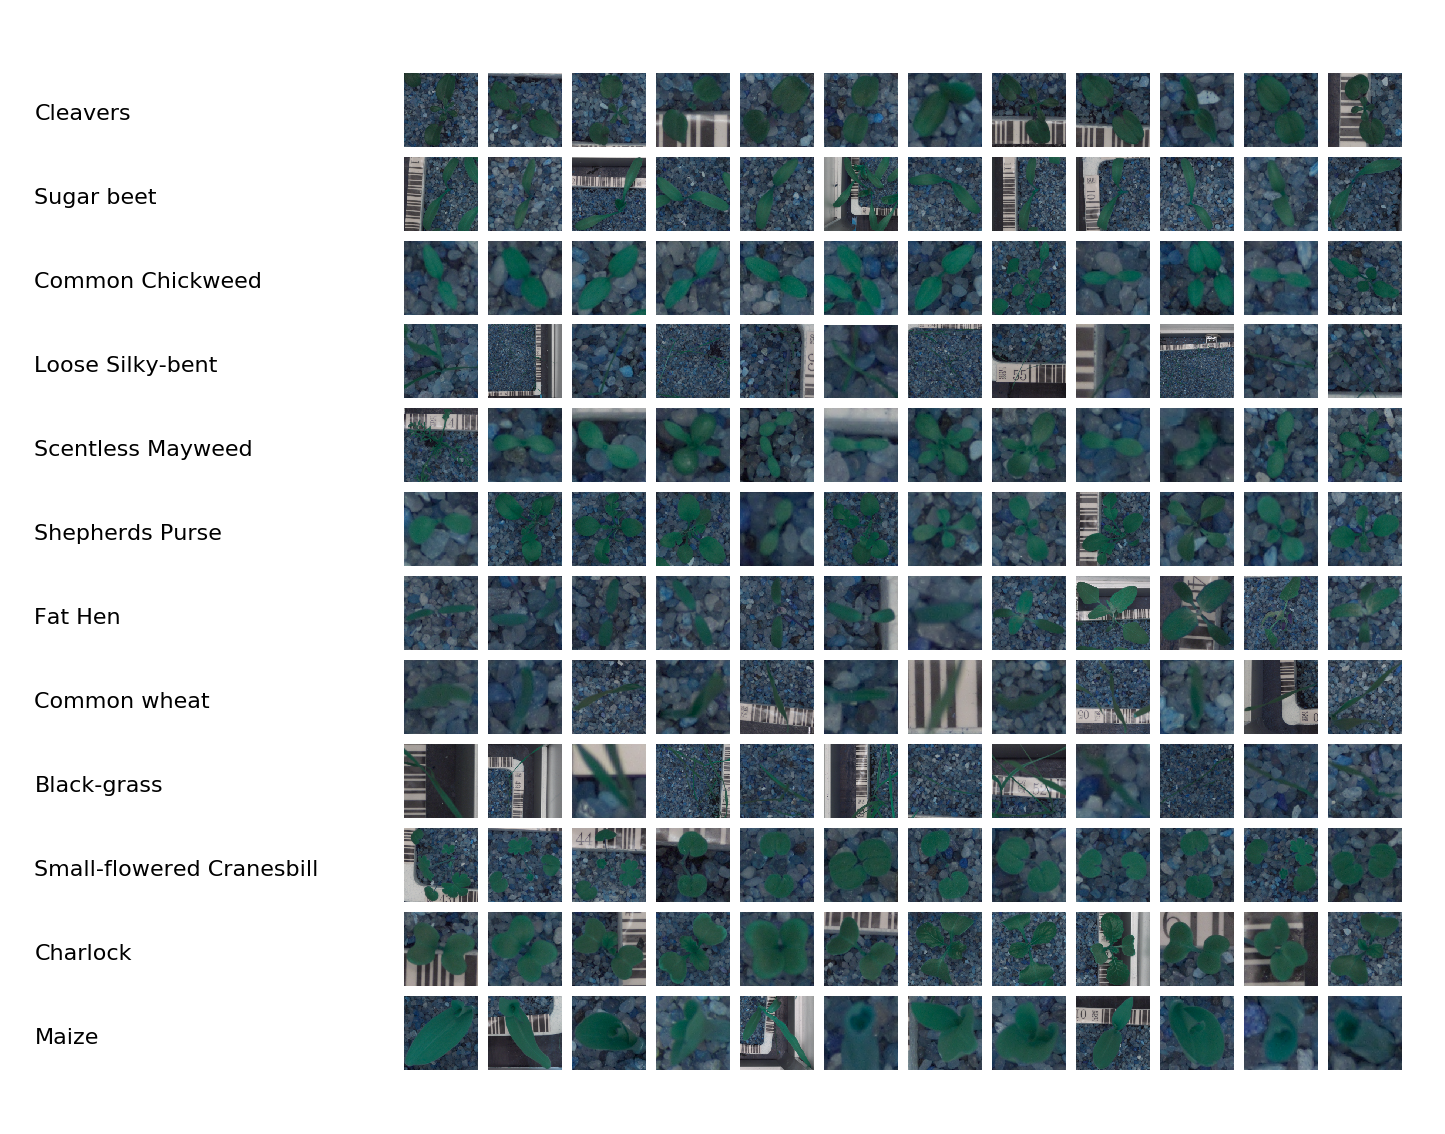
\includegraphics[height=7.5cm, width=10cm]{first_view_grid_1}
    \caption{Data overview}
    \label{fig:1}
\end{figure}

\subsection{Data preprocessing}

\subsection{Feature selection?}

\subsection{Classification}
